\documentclass[a4paper]{article}
\usepackage{graphicx}
\usepackage[margin = 1in]{geometry}
\usepackage{ragged2e}
\usepackage[hidelinks, colorlinks = true, citecolor = black, linkcolor = blue]{hyperref}
\usepackage{parskip}
\usepackage{cite}
\usepackage{caption}
\usepackage{subcaption}
\usepackage{cellspace}
\usepackage{makecell}
\usepackage{mwe}
\setlength\cellspacetoplimit{4pt}
\setlength\cellspacebottomlimit{4pt}
\usepackage{caption} 
\usepackage{pgfplots}
\usepackage{amsmath}
\usepackage{tikz}
\usepackage{pdfpages}
\newcommand{\inv}{^{\raisebox{.2ex}{$\scriptscriptstyle-1$}}}
\newcommand{\unit}[1]{~\mathrm{#1}}
\captionsetup[table]{skip=10pt}
\renewcommand{\arraystretch}{1.5}
\pgfplotsset{compat=1.16}
\pgfplotsset{ignore zero/.style={%
  #1ticklabel={\ifdim\tick pt=0pt \else\pgfmathprintnumber{\tick}\fi}
}}

\begin{document}
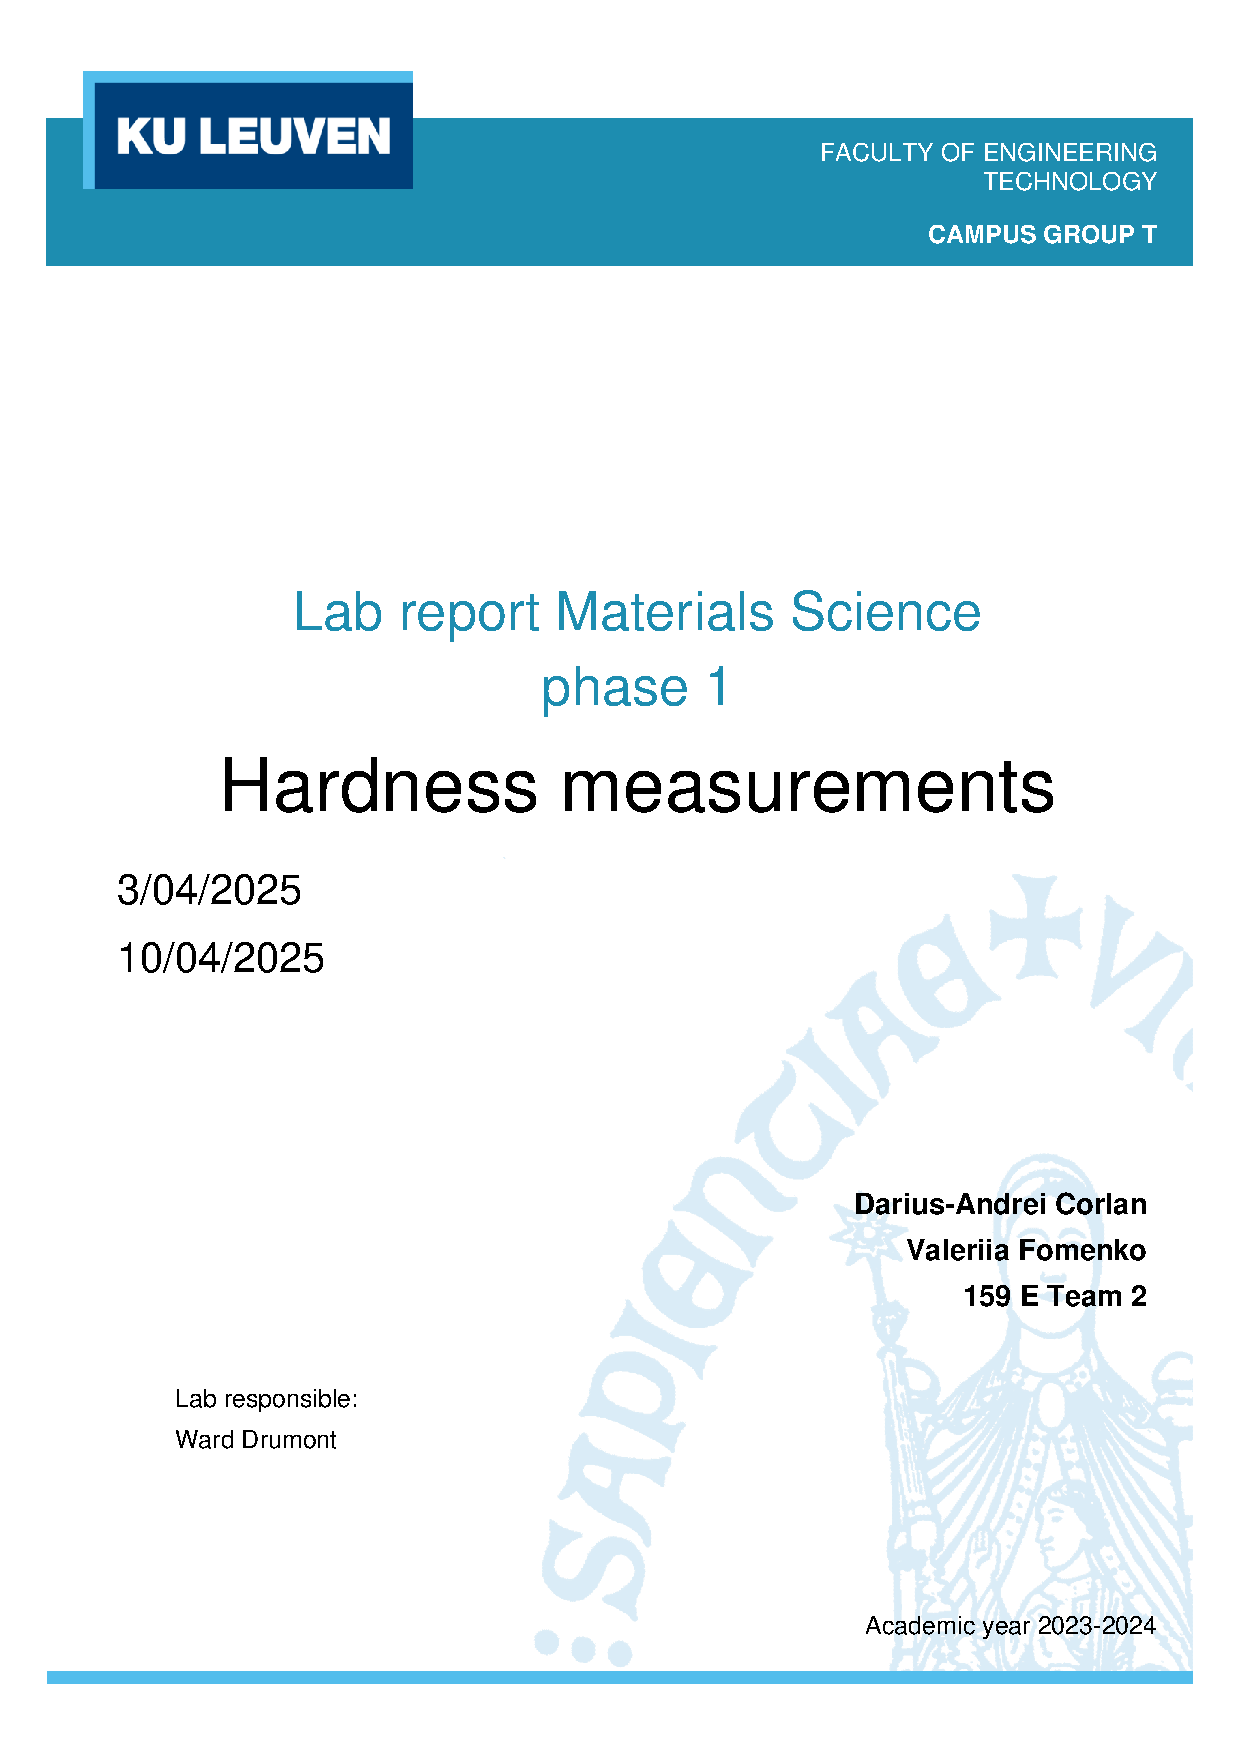
\includepdf[pages = {1}]{template.pdf}
\section{Introduction}
The objective of this experiment is to determine and compare the hardness of
various metal samples using the Brinell, Vickers, and Rockwell methods. The
lab focuses on evaluating the influence of material treatment such as
quenching and plastic deformation on hardness. Appropriate loads and indenters
are applied for each method, and multiple indentations are conducted to ensure
accuracy.

Results are analyzed using standardized conversion tables\cite{ASTME140} to establish correlations between hardness and tensile strength, as well as to assess the suitability of each testing method for different materials and applications.

\section{Background/ Theory}

The hardness of metals is measured via standardized tests, in which a small
indenter of a defined shape is pressed into the material with a certain force.
The hardness is then deduced from the dimensions of the indentation remaining
after the test (Vickers and Brinell methods)\cite{ASTME10,ASTME18}. In the Rockwell methods,
the hardness is read directly from the device on a dial gauge, which actually measures the
depth of this indentation.

\section{Method \& Materials}

A hardness apparatus is used for the test, in which one mounts the desired indenter, and one adjusts the desired force. A pre-load of 10 kgf is manually
applied to the sample beforehand by turning a wheel, pushing the sample against
the indenter with a force of 10 kgf. The rest of the measurement is performed
automatically: via a mechanism, the main load is applied, held for a few
seconds, and then removed.

5 total samples were tested using multiple types of hardness tests \textemdash~two
C-45 steel blocks, one of them being quenched, a brass strip, and two steel
tensile samples, one of them having undergone a tensile test. Before testing, we
polished the C-45 steel blocks using progressively smoother sandpaper. Firstly, the two
C-45 steel cubes and the brass strip are subjected to the Vickers hardness test.
Afterwards, all the samples get subjected to the two Rockwell tests. To
determine which rockwell test would be appropriate, the Vickers rating is used.
Finally, the brass sample is subjected to the Brinell test. 
\newpage

\section {Results}

\subsection{Measurements}
\subsubsection{Vickers measurements}
All of the samples were subjected to a load of $100\unit{kgf}$ and measured with a digital microscope which was able to digitally
measure the dimensions of the indentation. The results of these measurements is
displayed in table 1.

\begin{table}[!ht]
  \centering
  \label{tab:1}
  \caption{Measurement results of Vickers hardness test}
  \begin{tabular}{c|cc} 

  Material     & \makecell{$d_1$\\ $\unit{(mm)}$}    & \makecell{$d_2$\\$\unit{(mm)}$}     \\ 
  \hline
  $\mathrm{Steel_{hardened_1}}$   & 0.488 & 0.498  \\
  $\mathrm{Steel_{hardened_2}}$    & 0.5   & 0.515  \\
  $\mathrm{Steel_{hardened_3}}$    & 0.499 & 0.5    \\
  $\mathrm{Steel_{unhardened_1}}$ & 1.09  & 1.118  \\
  $\mathrm{Steel_{unhardened_2}}$  & 1.067 & 1.085  \\
  $\mathrm{Steel_{unhardened_3}}$  & 1.08  & 1.09   \\
  $\mathrm{Brass_1}$        & 1.06  & 1.054  \\
  $\mathrm{Brass_2}$        & 1.061 & 1.048  \\
  $\mathrm{Brass_3}$        & 1.06   & 1.058   \\

  \end{tabular}
  \end{table}

Afterwards, the necessary calculations are done to determine the Vickers
hardness, and the results are placed in table 2.

\begin{table}[!ht]
  \centering
  \label{tab:2}
  \caption{Hardness value results of the Vickers test}
  \begin{tabular}{c|cccc} 
  Material     & \makecell{$d_{avr}$\\$\unit{(mm)}$}    & \makecell{$HV_{avr}$ \\ $\unit{(-)}$}       & \makecell{$\Delta
  HV$\\ $\unit{(-)}$}   & \makecell{$HV_{standard ~notation}$ \\ $\unit{(-)}$}  \\ 
  \hline
  $\mathrm{Steel_{hardened}}$   & 0.5 & 741.33 & 20 & $(741.33 \pm 20)$   \\
  $\mathrm{Steel_{unhardened}}$ & 1.09    & 156.12 & 30 & $(156.12 \pm 30)$   \\
  $\mathrm{Brass}$        & 1.06 & 166.33 & 30 & $(166.33 \pm 30)$   \\

  \end{tabular}
  \end{table}

\subsubsection{Rockwell measurements}
By using the results of the Vickers hardness test, the kind of Rockwell test
that needed to be used was determined. For the hardened steel, Rockwell C (HRC) was
used, whereas for the brass and the unhardened steel, Rockwell B (HRB) was used.

\newpage
The results of the respective tests are arranged in table 3.

\begin{table}[!ht]
  \centering
  \label{tab:3}
  \caption{Rockwell hardness results for both of the steel blocks and brass strip}
  \begin{tabular}{c|ccc} 
  Measurement & \makecell{$\mathrm{Steel_{hardened}}$\\$\unit{(HRC)}$} &
  \makecell{$\mathrm{Steel_{unhardened}}$\\$\unit{(HRB)}$} & \makecell{$\mathrm{Brass}$\\ $\unit{(HRB)}$}  \\ 
  \hline
  1           & 67         & 80         & 86     \\
  2           & 62         & 82         & 86     \\
  3           & 63         & 81         & 87     \\
  4           & 61         & 83         & 87     \\
  5           & 83         & 84         & 88     \\
  \end{tabular}
  \end{table}

After taking the average of these values and calculating the error, the final
results are displayed in table 4.

\begin{table}[!ht]
  \centering
  \label{tab:4}
  \caption{Final result of the Rockwell hardness tests}
  \begin{tabular}{c|ccc}
  Material    & \makecell{$HR_{avr}$ \\ $\unit{(-)}$} & \makecell{$\Delta HR$ \\
  $\unit{(-)}$}  & \makecell{$HR_{standard~notation}$ \\ $\unit{(-)}$}  \\ 
  \hline
  $\mathrm{Steel_{hardened}}$   & 63.2  & 2 & $(63.2 \pm 2)$       \\
  $\mathrm{Steel_{unhardened}}$ & 82    & 1 & $(82 \pm 1)$       \\
  $\mathrm{Brass}$       & 86.8  & 1 & $(86.8 \pm 1)$      
  \end{tabular}
\end{table}

\subsubsection{Rockwell B measurements}
For both tensile samples, the Rockwell B hardness test was used. The
measurements are displayed in table 5.

\begin{table}[!ht]
  \centering
  \label{tab:5}
  \caption{All measurement results of the tensile samples}
  \begin{tabular}{c|cc}
  Measurement & \makecell{$\mathrm{Sample_{original}}$\\ $\unit{(-)}$} &
  \makecell{$\mathrm{Sample_{drawn}}$ \\ $\unit{(-)}$}  \\ 
  \hline
  1           & 65        & 82         \\
  2           & 61        & 86         \\
  3           & 69        & 87         \\
  4           & 58        & 86         \\
  5           & 61        & 87        
  \end{tabular}
\end{table}

Afterwards, the same steps to calculate the error are done as before, the final
results being displayed in table 6.

\begin{table}[!ht]
  \centering
  \label{tab:6}
  \caption{Final results of the tensile sample tests}
  \begin{tabular}{c|ccc}
  Material & \makecell{$HR_{avr}$\\$\unit{(-)}$} & \makecell{$\Delta HR$ \\
  $\unit{(-)}$}  & \makecell{$HR_{standard~notation}$ \\ $ \unit{(-)}$}  \\ 
  \hline
  $\mathrm{Sample_{drawn}}$ & 85.6  & 2 & $(85.6 \pm 2)$       \\
  $\mathrm{Sample_{original}}$ & 82    & 1 & $(82 \pm 1)$      
  \end{tabular}
\end{table}

\newpage
\subsubsection{Brinell for brass}
To perform the Brinell test, first the load force has to be calculated.
The force is determined to be $60\unit{kgf}$. Afterwards, the results of the
indentation measurements are noted down in table 7.

\begin{table}[!ht]
  \centering
  \label{tab:7}
  \caption{Indentation results of the Brinell test}
  \begin{tabular}{c|c}
  Measurement & \makecell{$d_{indentation}$\\ $\unit{(mm)}$}      \\ 
  \hline
  1           & 0.728  \\
  2           & 0.709  \\
  3           & 0.719  \\
  4           & 0.728  \\
  5           & 0.72  
  \end{tabular}
\end{table}

Finally, the final hardness value can be calculated. The results of this
calculation are shown in table 8.

\begin{table}[!ht]
  \centering
  \label{tab:8}
  \caption{Hardness measurement results of the Brinell test}
  \begin{tabular}{c|ccc}
  \makecell{$d_{avr}$ \\ $\unit{(mm)}$}   & \makecell{$HB_{avr}$ \\
  $\unit{(-)}$}  & \makecell{$\Delta HB$ \\ $\unit{(-)}$} &
  \makecell{$HB_{standard~notation}$ \\ $\unit{(-)}$}  \\ 
  \hline
  0.721 & 150 & 20     & $(150 \pm 20)$    
  \end{tabular}
\end{table}

\subsection{Calculations}
\subsubsection{Vickers measurement}
Eq. (1) calculates the Vickers hardness number (HV) by dividing the applied load
(P) by the square of the average diagonal length (d) of the indentation, scaled
by a constant factor (1.85) to account for the geometry of the diamond pyramid
indenter\cite{LoeckxHardness}.
\begin{equation}
  HV = 1.85 \cdot \frac{P}{d^2}
\end{equation}

A calculation for the first test of the vickers indentation is:

\[HV = 1.85 \cdot \frac{100}{0.493^2} = 762.8\]

Because Vickers hardness depends on the square of the diagonal length, a
relative error in the diagonal measurement results in twice that relative error
in the calculated hardness value\cite{LoeckxHardness}:

\begin{equation}
  \Delta HV = HV(\sqrt{2} \cdot \frac{\Delta d}{d})
\end{equation}


To calculate the error of the diameter, both the spread of the indentation
diameters and the error of the digital microscope must be taken into account\cite{LoeckxHardness}.
The formula used is shown in Eq. (3).

\begin{equation}
  \delta d = \sqrt{\left( \frac{\frac{2 s_d}{\sqrt{n}}}{d_{indent}} \right )^2 + 0.01^2}
\end{equation}

By using this equation, the error of the indentation diameter can be calculated:

\[ \delta d = \sqrt{\left( \frac{\frac{2 \cdot 0.0085
}{\sqrt{3}}}{1} \right )^2 + 0.01^2} = 0.1 \]


Therefore, the error of the Vickers hardness test can be calculated:    
      
\[ \Delta HV = HV_{avr} (\sqrt{2}\cdot 0.1) = 14.6  \approx 20\]

Afterwards, the error rounded to one significant digit to maintain consistency
between different types of measurements\cite{DeneyerUncertainty}, concluding to
a final result of:
\[HV = (741.3 \pm 20)\]

\subsubsection{Rockwell measurements}
Since the Rockwell measurement results are displayed directly on the hardness
testing machine, only the error on the measurement needs to be determined. This
is done using the method for determining standard error using standard
deviation\cite{DeneyerUncertainty}. Firstly, the standard deviation needs to be determined. This is
done using Microsoft Excel's standard deviation formula. Afterwards the error is
determined using Eq. (4).

\begin{equation}
  \Delta HRB = \frac{s}{\sqrt{n}}
\end{equation}

By using this equation with the measurements for the drawn tensile sample, the
following calculation ensues:

\[ \Delta HRB = \frac{2.94}{\sqrt{5}} = 1.316 \approx 2\]

Contributing to a final result of:

\[ HRB = (85.6 \pm 2)\]

\subsubsection{Brinell for brass}
Eq. (5) determines the Brinell hardness number (HB) by calculating the applied
load (P) divided by the curved surface area of the indentation, based on the
indenter diameter (D) and the measured indentation diameter (d)\cite{LoeckxHardness}.

\begin{equation}
  HB = \frac{2P}{\pi D(D-\sqrt{D^2 - d^2})}
\end{equation}

By using the average diameter value, the Brinell hardness can be calculated:
\[ HB = \frac{2\cdot 60}{\pi \cdot 2.5(2.5 - \sqrt{2.5^2 - 0.721^2})} = 150.2\]

Finally, to calculate the error of the Brinell test, the error of the diameter
measurement must be calculated. By using Eq. (3), the following calculation
is made:

\[\delta d = \sqrt{\left( \frac{\frac{2 \cdot 0.00786
}{\sqrt{5}}}{2.5} \right )^2 + 0.01^2} = 0.1\]

Afterwards Eq. (2) can be used to calculate the error of the Brinell test
measurements:

\[\Delta HB = 150.15 (\sqrt{2} \cdot 0.2) = 15.02 \approx 20\]

Contributing to a final result of:

\[ HB = (150.15 \pm 20)\]

\section{Discussion}

The primary goal of the experiment was to investigate the hardness of different metal samples using Vickers, Brinell, and Rockwell hardness testing methods. Particular attention was given to understanding the influence of quenching and plastic deformation on steel hardness. Additionally, the suitability, precision, and consistency of each method were evaluated.

\subsection{Consistency of Results and Method Comparison}

The obtained results, summarized in Table 9 below, demonstrate overall
consistency across the methods when conversion relationships are taken into
account.

\begin{table}[!ht]
  \centering
  \label{tab:9}
  \caption{Overview of measured hardness values}
  \begin{tabular}{c|ccc}
  Material                  & Vickers (HV) & Rockwell (HRB/HRC) & Brinell (HB)  \\ 
  \hline
  $\mathrm{Steel_{unhardened}}$         & $(156.1 \pm 30)$   & $(82 \pm 1)$ HRB         & -             \\
  Steel, hardened           & $(741.3 \pm 20)$  & $(63.2 \pm 2)$ HRC       & -             \\
  Brass                     & $(166.3 \pm 30)$   & $(86.8 \pm 1)$ HRB       & $(150.1 \pm 20)$      \\
  Tensile sample (original) & -            & $(82 \pm 1)$ HRB         & -             \\
  Tensile sample (drawn)    & -            & $(85.6 \pm 2)$ HRB       & -            
  \end{tabular}
  \end{table}

  The results for the brass sample confirm mutual consistency among the three testing methods. The Vickers value (166 HV) corresponds well with the Brinell result (150 HB), and the Rockwell B reading (86.8 HRB) falls within the expected range based on the Vickers-to-Rockwell conversion chart(labtexgt).

  In the case of steel samples, the large disparity in hardness values between the hardened and unhardened C45 blocks validates the significant effect of quenching. Quenching transformed the steel’s microstructure to martensite, which is much harder and more brittle\cite{DewolfMaterials}. This was reflected in the increase of the Vickers hardness from approximately 156 HV to 741 HV, and a corresponding shift from HRB 82 to HRC 63. These transitions align with the theoretical expectations and provided conversion tables\cite{ASTME140}.
  
  The Rockwell B values for the tensile samples (original and drawn) also illustrate the phenomenon of work hardening. The drawn sample exhibited a hardness of 85.6 HRB compared to 82 HRB for the original, indicating an increase in strength due to dislocation multiplication during plastic deformation.
  
  \subsection{Accuracy and Precision of the Methods}
  
  Among the methods, Vickers showed the highest potential accuracy due to its
  diamond indenter and independence from applied load. However, its results also
  demonstrated the highest uncertainty, primarily due to the microscope's
  limited resolution and the squared dependence of the formula on diagonal
  length, amplifying any small error in measurement. By using a digital
  microscope, the precision of this test is limited by the scale of the diameter
  measurement.
  
  The Brinell method, although robust and suited for heterogeneous materials like brass, showed a moderate error of ±20. This is attributed to the difficulty in precisely measuring the indentation diameter and the need for surface preparation.
  
  Rockwell tests proved the most practical and precise (±1 to ±2) due to their direct digital readings and minimal user interpretation\cite{astme18}. They are thus particularly suitable for routine testing in industrial contexts.
  
  \subsection{Interpretation of Deviations}
  
  No significant discrepancies were observed among the methods when accounting
  for conversion and material suitability. 
  \newpage
  
  \subsection{Answers to the questions}
  \begin{enumerate}
    \item \textbf{Hardness–Tensile Strength Relation:}
    
    The approximate empirical formula is:
    \begin{equation}
      \sigma _{ts} \approx 3.45 HV
    \end{equation}
    \item \textbf{Why Not Start With Brinell or Rockwell B:}
    
    Brinell and Rockwell B are inappropriate for very hard materials. Starting
    with them may damage the steel indenter or yield no indentation. Vickers,
    with its diamond indenter, is safer for unknown hardness levels.
    \item \textbf{Recommended Methods:}
    
    \begin{itemize}
      \item Thin copper plates: Vickers — due to the small indentations and minimal load required.
      \item Hardened steel in series production: Rockwell C — fast, repeatable, and directly readable.
      \item Cast bronze bearing: Brinell — larger indenter averages out local inhomogeneities.
    \end{itemize}
    \item \textbf{Why So Many Hardness Methods:}
    
    Different materials and applications require different penetrative forces,
    sensitivities, and surface preparations. Brinell suits coarse materials,
    Vickers small or thin specimens, Rockwell provides fast results, and each
    method suits a specific industrial context.
    
    \item \textbf{Rockwell Method for Brinell 175:}
    
    According to the conversion graph, a Brinell hardness of 175 corresponds to
    approximately 89.6 HRB. Thus, Rockwell B is appropriate.

    \item \textbf{Why Not Indent Too Close:}
    
    A second indentation near a previous one affects the stress distribution,
    typically causing the material to appear softer (measured value too low) due
    to local work hardening and plastic deformation already induced.
    
    \item \textbf{Hardness of Rubber – Shore Hardness:}
    
    The Shore durometer test uses a spring-loaded indenter to measure resistance to penetration. It differs fundamentally from metal hardness tests by being dynamic and dependent on elastic rather than plastic deformation\cite{ASTMD2240}.
  \end{enumerate}

\section{Conclusion}
The experiment confirmed the substantial effect of heat treatment on hardness,
with quenched C45 steel exhibiting a hardness of $(741 \pm 20)\unit{HV}$
compared to $(156 \pm 30)\unit{HV}$ for unhardened steel. Rockwell tests provided the most
repeatable
results $\mathrm{(\pm 1–2)\unit{HRB/HRC}}$, while Vickers and Brinell methods showed higher
uncertainties due to measurement sensitivities. These findings highlight the
need to align hardness testing methods with material properties:Vickers for
precision on small features, Rockwell for rapid industrial use, and Brinell for
coarse or inhomogeneous materials.
\section{Bibliography}
\bibliographystyle{IEEEtran}
\bibliography{SBSM}
\end{document}

